\documentclass[11pt]{article}

\usepackage[a4paper,margin=1in]{geometry}
\usepackage{amsmath}
\usepackage{amssymb}
\usepackage{booktabs}
\usepackage[round,authoryear]{natbib}
\usepackage{hyperref}
\usepackage{tikz}
\usepackage{graphicx}
\usepackage{longtable}
\usepackage{pdfpages}
\usetikzlibrary{arrows.meta,positioning,fit,backgrounds,calc,decorations.pathreplacing}

\hypersetup{colorlinks=true,linkcolor=black,citecolor=blue,urlcolor=blue}

\newcommand{\E}{\mathbb{E}}
\newcommand{\R}{\mathbb{R}}
\newcommand{\code}[1]{\texttt{\small #1}}

\title{\textbf{A Real-Time Global Scenario System for Policy Analysis:\\
An EM--Bayesian GVAR with an Endogenous United States}\\[4pt]
\large{(Working draft)}}
\author{M.\ Farkas}
\date{\today}

\begin{document}
\maketitle

\begin{abstract}
\noindent Policy analysts often need to answer a simple question, and answer it quickly: if one thing
changes, what happens to the rest of the world? We build a tool that answers it. The user fixes a few
variables---a policy rate, a credit spread, a path for the budget---and the tool reports how growth,
inflation, interest rates, and public debt respond across $50$ economies. It runs in a web browser and
updates in a fraction of a second, so the user can try one scenario after another during a meeting.

Behind the tool is a single model: a set of country vector autoregressions, estimated with Bayesian
shrinkage and tied together by trade. Three choices make it work in practice. First, we fill in the
missing data---short samples and the pandemic quarters---\emph{inside} the estimation, rather than
cleaning the data beforehand. Second, we let the United States respond to the rest of the world, instead
of holding it fixed as an anchor the way the standard global VAR does. Third, we use one simple fact:
once the model is estimated, a scenario is a linear problem. That lets us compute the answer to any
scenario once and reuse it, which is why the tool is fast.

We ask the model two questions. Does it forecast well? In a real-time contest over roughly $2013$--$2024$
against eight competitors, it does not win on point accuracy---a factor model and a simple autoregression
do---but on growth, inflation, and interest rates it belongs to the set of best models by a formal test
(the Model Confidence Set), and it significantly beats, on growth and inflation, the textbook global VAR it
generalizes. Its probability bands come out too narrow, which we report openly. What does it add as a
scenario tool? A US interest-rate scenario spreads to every economy in a single solve, and because the US
now responds to the rest of the world, the model captures a feedback onto the US that the fixed-anchor
version cannot. The contribution is the whole system: one model that both forecasts and supports
transparent, fast, multi-country scenario analysis.
\end{abstract}

%% =====================================================================
\section{Introduction}
%% =====================================================================

Suppose the Federal Reserve is about to raise interest rates. An analyst needs to know what this does to
growth and inflation in the euro area, in Mexico, in the rest of the world---and what it does back to the
United States. Or suppose corporate credit spreads jump, or a government loosens its budget. Questions
like these come up every day in central banks, finance ministries, and international organizations.
Answering one well needs a model with four properties at once: it is global, so it covers many countries
together; it is disciplined, so it is small enough to estimate reliably; it is honest about messy data;
and it is fast enough to re-run while the discussion is still going. No standard tool has all four.

This paper builds and documents a tool that does. The user fixes a few variables---say, a path for the US
policy rate---and the tool returns the response of every variable in every one of $50$ economies,
consistent with the estimated model and with how the economies are linked. It runs in an ordinary web
browser and re-solves in well under a second, so the user can explore one scenario after another. The
tool is live and in use; this paper explains what is inside it and shows that it works.

Inside the tool is a single model. Its starting point is standard: a vector autoregression for each
economy, estimated with Bayesian shrinkage \citep{Litterman1986,GiannoneLenzaPrimiceri2019}, with the
economies linked through trade-weighted averages of their partners' variables, as in the global VAR
literature \citep{PesaranSchuermannWeiner2004,DeesDiMauroPesaranSmith2007}. Three choices make it work in
practice. First, we fill in the missing data---short emerging-market samples and the pandemic
quarters---as part of the estimation, using a Kalman smoother, rather than cleaning the data beforehand
\citep{DurbinKoopman2012,LenzaPrimiceri2022}. Second, we let the United States respond to the rest of the
world, instead of holding it fixed as an anchor, which is how classical global VARs treat the dominant
economy. Third, we add a small fiscal block for six large economies, so a scenario carries its
public-debt implications automatically.

The step that turns this model into an interactive tool is a piece of algebra. Once the model is
estimated, imposing a scenario is a linear problem: the response of the whole system is a fixed, known
function of the numbers the user pins down. We solve that linear problem once, offline, and store the
answer, so that during use each new scenario is a single matrix multiplication. This is why a
$50$-economy model can re-solve in a browser in a fraction of a second.

We then ask whether the model is any good, and we are strict about it. In a real-time forecasting contest
over roughly $2013$--$2024$ against eight competitors---from a random walk up to the textbook global
VAR---the model does not win on point accuracy: a factor model forecasts growth best, and a simple
autoregression forecasts inflation and interest rates best. But by a formal test of forecast accuracy it is
statistically among the best models on growth, inflation, and interest rates, and it significantly beats
the textbook global VAR it generalizes on growth and inflation, so the extra machinery earns its place.
One weakness is visible and we report it plainly: the model's probability bands come out too narrow.

Finally we show what the tool adds. A US interest-rate scenario spreads coherently to every economy in a
single solve, and the tool shows the debt consequences next to the growth-and-inflation response. Because
we let the United States respond to the rest of the world, the model also captures a feedback from abroad
back onto the US that a fixed-anchor global VAR cannot produce; we measure its size, while being clear
that this is a scenario projection, not a causal impulse response.

The contribution is the system as a whole. None of the individual ingredients is new; carrying all of
them in one estimated model that both forecasts credibly and answers scenario questions in real time,
from a single reproducible set of files, is. The rest of the paper follows the tool.
Section~\ref{sec:glance} sketches the architecture; Section~\ref{sec:estimation} explains how the model is
estimated; Section~\ref{sec:engine} explains how it is solved and used in real time;
Section~\ref{sec:data} describes the data and is candid about its limits; Section~\ref{sec:horserace} is
the forecasting test; Section~\ref{sec:scenario} is the scenario application; Section~\ref{sec:discussion}
discusses what the tool enables and where it falls short; Section~\ref{sec:conclusion} concludes.

%% =====================================================================
\section{The system at a glance}
\label{sec:glance}
%% =====================================================================

The tool has three parts (Figure~\ref{fig:system}): a set of country models, a layer that links them
through trade, and a layer that solves and conditions the linked system in real time. The first two parts
are about estimating the model; the third is what turns it into an interactive tool. The paper is
organized the same way---Section~\ref{sec:estimation} covers the first two parts, Section~\ref{sec:engine}
the third---and this section gives the map.

\begin{figure}[t]
\centering
\resizebox{\textwidth}{!}{%
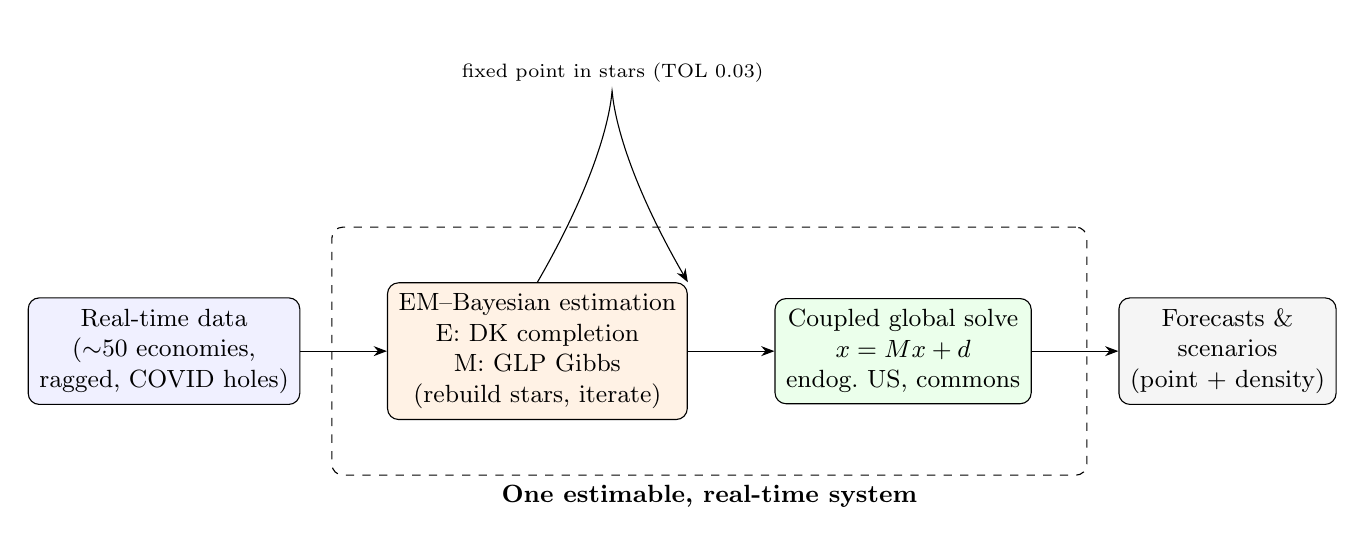
\begin{tikzpicture}[
  >=Stealth, node distance=9mm and 11mm, font=\small,
  box/.style={draw, rounded corners, align=center, minimum height=10mm, inner sep=4pt, fill=white},
  data/.style={box, fill=blue!6},
  est/.style={box, fill=orange!10},
  solve/.style={box, fill=green!8},
  fout/.style={box, fill=gray!8}
]
  \node[data] (data) {Real-time data\\ ($\sim$50 economies,\\ ragged, COVID holes)};
  \node[est, right=of data] (em) {EM--Bayesian estimation\\ E: DK completion\\ M: GLP Gibbs\\ (rebuild stars, iterate)};
  \node[solve, right=of em] (solve) {Coupled global solve\\ $x = Mx + d$\\ endog.\ US, commons};
  \node[fout, right=of solve] (out) {Forecasts \&\\ scenarios\\ (point + density)};
  \draw[->] (data) -- (em);
  \draw[->] (em) -- (solve);
  \draw[->] (solve) -- (out);
  \draw[->] (em.north) to[out=60,in=120,looseness=5] node[above,font=\scriptsize,align=center]{fixed point in stars (TOL $0.03$)} (em.north east);
  \begin{scope}[on background layer]
    \node[draw, dashed, rounded corners, fit=(em)(solve), inner sep=7mm, label=below:{\textbf{One estimable, real-time system}}] {};
  \end{scope}
\end{tikzpicture}}
\caption{The three layers: real-time data $\to$ EM--Bayesian estimation (layers one and two, coupled and
completed inside one fixed point) $\to$ the coupled global solve $x=Mx+d$ (layer three) $\to$
forecasts and scenarios. The dashed box is the single estimable object; the solve layer is what makes it
an interactive tool.}
\label{fig:system}
\end{figure}

The first part is a separate model for each economy. Each is a vector autoregression---a set of equations
in which this quarter's variables depend on the last three quarters'---covering output, prices, the
labour market, interest rates, credit, the exchange rate, and, for $42$ economies, the public finances.
The models range from $16$ variables (a small emerging market) to $40$ (the United States, which also
carries the globally-traded prices and its own foreign-feedback terms); across the $50$ economies there
are $1{,}182$ estimated series in all. Each model is small enough to estimate reliably yet detailed
enough to answer a policy scenario.

The second part links the economies through trade. Each economy sees three summaries of the rest of the
world---its trading partners' growth, inflation, and interest rate, each partner weighted by how much the
economy trades with it---together with four globally-traded prices set mainly in US markets: oil, the US
long-term interest rate, a US corporate borrowing spread, and US equity. Two features matter. Summarizing
the rest of the world in three trade-weighted numbers, rather than tracking every foreign variable, is
what keeps a $50$-economy system estimable. And, unlike the standard global VAR, the United States is one
of the linked economies rather than an outside anchor, so a shock abroad can feed back onto it.

The third part solves and conditions the linked system in real time. Because a scenario is a linear
problem once the model is estimated (Section~\ref{sec:engine}), the answer can be pre-computed once and
reused, so any constraint the user imposes on any economy re-solves all $50$ at once, instantly. This is
the part that makes the model a tool rather than a batch forecaster.

We use the following notation throughout. There are $33$ trade-linked economies plus $17$ euro-area
members estimated on their own (they take the euro-area interest rate and related series as external
inputs); six economies (US, EA, JP, UK, CA, CN) carry a public-finance block. Each model uses three lags
($p=3$) and is forecast $20$ quarters ahead ($H=20$). Stacked together, the linked system has about
$2{,}060$ dimensions and is stable, in the sense that shocks die out rather than build up (its largest
eigenvalue is $0.947$, below one). We write $y_{i,t}$ for economy $i$'s own variables and $y^{*}_{i,t}$
for its three foreign summaries, and leave the details of each part to the sections that follow.

%% =====================================================================
\section{The EM--Bayesian GVAR}
\label{sec:estimation}
%% =====================================================================

This section details the engine: how the fused object of layers one and two is estimated as a single
fixed point. We build it up in the order the estimator runs---the per-bloc Bayesian VAR and its prior
(\S\ref{sub:blocs}), the trade-weighted coupling (\S\ref{sub:stars}), the EM data-completion that makes
ragged and pandemic-scarred panels usable (\S\ref{sub:em}), the endogenous dominant unit
(\S\ref{sub:endous}), the fiscal block (\S\ref{sub:fiscal})---and close with the fixed point that ties
them together (\S\ref{sub:fixedpoint}).

\subsection{Per-country Bayesian VARs and the GLP prior}
\label{sub:blocs}

Each economy is a reduced-form VAR whose coefficients are shrunk by a hierarchical Minnesota/GLP prior
with data-driven tightness. Stacking economy $i$'s domestic variables $y_{i,t}$ with its three
trade-weighted foreign stars $y^{*}_{i,t}$ into $x_{i,t} = [\,y_{i,t}'\;\; y^{*\prime}_{i,t}\,]'$,
\begin{equation}
  x_{i,t} = c_i + \sum_{\ell=1}^{p} A_{i,\ell}\,x_{i,t-\ell} + u_{i,t},
  \qquad p = 3,\quad u_{i,t}\sim\mathcal{N}(0,\Sigma_i).
  \label{eq:bloc}
\end{equation}
Variables enter in one of two spaces: levels in $100\log$ for real quantities and price indices (whose
displayed growth is $4\,\Delta$), and raw levels for rates and ratios; the ``factor of four, not four
hundred'' quarterly-annualised convention is fixed once and used everywhere.

A bloc with up to $40$ variables and three lags has too many coefficients to estimate freely on a short
sample, so we discipline them with a prior. The prior pulls each equation toward a simple benchmark---a
random walk, in which each variable's best forecast is its current value---and lets the data pull away
from that benchmark only where the evidence is strong. How hard it pulls is not chosen by hand but learned
from the data: this is the hierarchical prior of \citet{GiannoneLenzaPrimiceri2019} and
\citet{Giannone2015}, governed by two numbers (an overall tightness $\lambda$, prior mode $0.2$, and a
sum-of-coefficients weight $\mu$, prior mode $1$). This learned shrinkage is what makes even the
short-sample emerging-market blocs estimable without dropping the cross-country links.

The hyperparameters are not fixed but sampled, which matters under missing data. Within each bloc's
Gibbs sampler, $(\lambda,\mu)$ are updated by a random-walk Metropolis--Hastings step on the
\emph{completed-data} marginal likelihood, initialised at the numerical optimum and with a proposal
covariance taken from the prior's inverse Hessian; the shrinkage therefore adapts to the imputed panel
rather than to a truncated balanced window. Because the same sampler also draws the missing cells
(\S\ref{sub:em}), estimation of the prior, the coefficients, and the data completion all condition on one
another.

A small but consequential prior choice concerns the fiscal ratios. Most variables carry the random-walk
prior mean natural to macro levels, but the estimated fiscal ratios---revenue and primary expenditure as
shares of GDP, and the stock--flow adjustment---carry a \emph{white-noise} (stationary) prior mean of
zero own-persistence, reflecting that a revenue-to-GDP ratio mean-reverts rather than drifts. The
effective interest rate, by contrast, retains the random-walk prior. This keeps the fiscal drivers'
long-run behaviour economically sensible and, as Section~\ref{sub:fiscal} shows, keeps the derived debt
path well-behaved.

\subsection{Cross-country coupling through trade-weighted stars}
\label{sub:stars}

The link between economies runs through three ``foreign'' variables per economy, each built from its
trading partners rather than taken from outside data. For economy $i$ we form a foreign growth, a foreign
inflation, and a foreign interest rate by averaging its partners' values, weighting each partner by how
much $i$ trades with it:
\begin{equation}
  y^{*}_{i,t}\;=\;\sum_{j\neq i} w_{ij,t}\, z_{j,t},
  \qquad
  w_{ij,t} = \frac{\bar w_{ij}\,\mathbf{1}\{j \in \mathcal{P}_{i,t}\}}{\sum_{k\neq i}\bar w_{ik}\,\mathbf{1}\{k\in\mathcal{P}_{i,t}\}},
  \label{eq:stars}
\end{equation}
where $z_{j,t}$ is partner $j$'s growth, inflation, or interest rate and $\bar w_{ij}$ is the trade
weight. Following the global-VAR literature we call these three foreign averages the \emph{stars}.
Summarizing the entire rest of the world in three numbers per economy, rather than carrying every foreign
variable, is the step that keeps a $50$-economy model estimable and, later, quick to solve.

We recompute the weights each quarter over the partners that actually have data that quarter---the set
$\mathcal{P}_{i,t}$ in \eqref{eq:stars}---which is what lets the model run on an unbalanced panel. If a
partner's series is missing (a country not yet in the sample, or one with no comparable interest rate) it
simply drops out of that quarter's average for that variable. The growth and inflation averages can draw
on a wider set of partners than the interest-rate average, which leaves out economies without a
comparable rate or with runaway inflation that would swamp it.

Alongside these three, four globally-traded prices enter every economy in the same way: oil, the US
ten-year interest rate, a US corporate borrowing spread, and US equity. For these a single world price,
set mostly in US markets, is the natural object, so we carry one series each rather than a separate copy
per economy. This saves parameters and imposes the sensible restriction that the oil price a scenario
feeds into Germany is the same one it feeds into Chile.

Figure~\ref{fig:topology} is the picture to keep in mind. Every economy is a small model in its own right;
the trade-weighted foreign averages (the two-way arrows) tie the economies together; and the four
globally-traded prices (the dashed arrows) reach all of them at once. The one feature that sets this
construction apart from the textbook global VAR is at the centre: the United States is a bloc like any
other, both sending shocks out to the world \emph{and} taking feedback back in, rather than sitting
outside the system as a fixed anchor.

\begin{figure}[t]
\centering
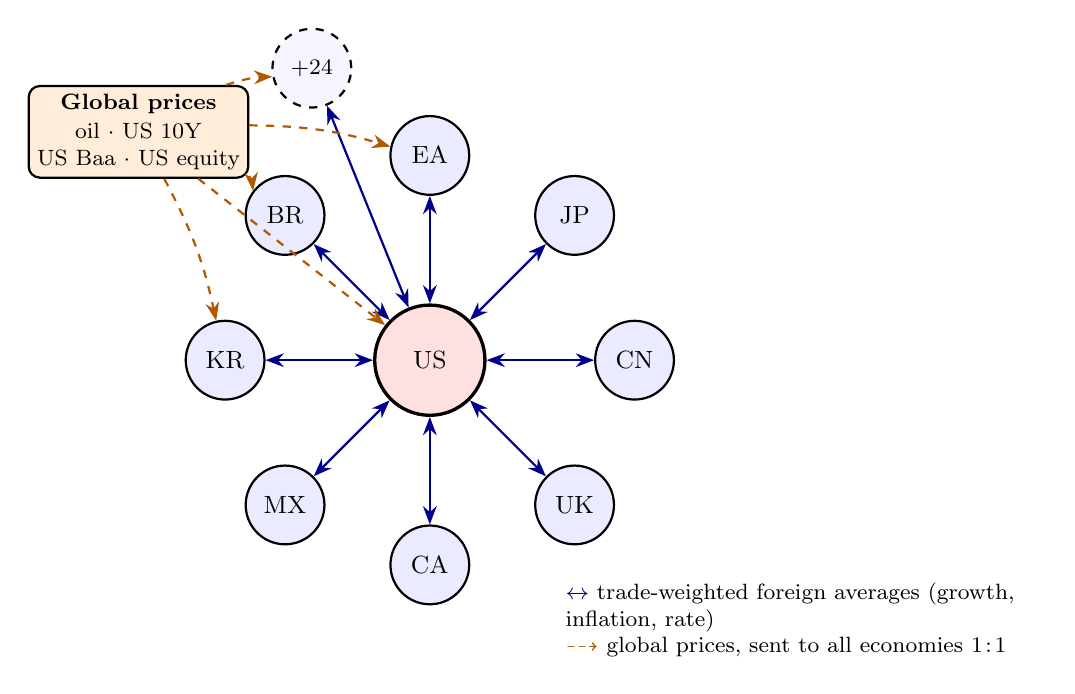
\begin{tikzpicture}[
  >=Stealth, font=\small,
  bloc/.style={circle, draw, thick, minimum size=10mm, inner sep=1pt, fill=blue!8},
  hub/.style={circle, draw, very thick, minimum size=14mm, inner sep=1pt, fill=red!12},
  commons/.style={rectangle, rounded corners, draw, thick, fill=orange!15, align=center, inner sep=3pt, font=\footnotesize},
  star/.style={<->, thick, blue!55!black},
  bcast/.style={->, thick, orange!70!black, dashed},
]
  \node[hub] (US) at (0,0) {US};
  \node[bloc] (EA) at ( 90:2.6) {EA};
  \node[bloc] (JP) at ( 45:2.6) {JP};
  \node[bloc] (CN) at (  0:2.6) {CN};
  \node[bloc] (UK) at (-45:2.6) {UK};
  \node[bloc] (CA) at (-90:2.6) {CA};
  \node[bloc] (MX) at (-135:2.6) {MX};
  \node[bloc] (KR) at (180:2.6) {KR};
  \node[bloc] (BR) at (135:2.6) {BR};
  \node[bloc, fill=blue!4, dashed] (more) at (112:4.0) {\footnotesize $+24$};
  \foreach \c in {EA,JP,CN,UK,CA,MX,KR,BR} {\draw[star] (US) -- (\c);}
  \draw[star] (US) -- (more);
  \node[commons] (GC) at (-3.7,2.9) {\textbf{Global prices}\\[1pt] oil $\cdot$ US 10Y\\ US Baa $\cdot$ US equity};
  \draw[bcast] (GC) -- (US);
  \foreach \c in {EA,BR,KR,more} {\draw[bcast] (GC) to[bend left=8] (\c);}
  \node[align=left, font=\footnotesize, anchor=west, text width=6.0cm] at (1.6,-3.3)
    {\textcolor{blue!55!black}{$\leftrightarrow$}\ trade-weighted foreign averages (growth, inflation, rate)\\
     \textcolor{orange!70!black}{$\dashrightarrow$}\ global prices, sent to all economies $1\!:\!1$};
\end{tikzpicture}
\caption{How the economies are linked. A central United States bloc is tied to the $32$ other economies
(eight labelled, plus $24$ more) through two-way, trade-weighted ``foreign average'' links carrying each
partner's growth, inflation, and interest rate; four globally-traded prices are broadcast to every economy
at once. Crucially the United States is a full member of the system, not a fixed anchor---it both drives
the rest of the world and responds to it. The resulting cross-country system is stable: the feedback
across economies has spectral radius $\rho(M)=0.947<1$ (against $0.70$ for the fixed-anchor version), so
the coupled solve of \S\ref{sub:affine} has a unique answer.}
\label{fig:topology}
\end{figure}

\subsection{EM data-completion under ragged and pandemic missingness}
\label{sub:em}

Our data have two kinds of holes, and we fill both as part of the estimation rather than patching them
beforehand. The first kind is ragged edges: economies enter the sample at different dates, so at any
quarter some series are simply not yet available. The second is the $2020$ pandemic, whose swings are so
large that leaving them in would distort the estimated dynamics. The usual fixes---cut every series back
to the shortest common sample, or delete the pandemic quarters---either throw away years of data or leave
a hole that the cross-country links then spread everywhere. Instead we treat each hole as missing data and
fill it with its best model-based estimate given everything else that is observed.

For the pandemic we make one specific choice, and it does most of the work. Over the three quarters
$2020$Q2--Q4 we treat the real-economy variables---output, prices, and the two real-economy foreign
averages---as missing, but keep the financial variables---interest rates, spreads, equity---as observed.
The reason is that financial markets kept pricing through the pandemic and so carry genuine information
about it. A Kalman smoother \citep{DurbinKoopman2012} then reconstructs the missing real-economy path from
that financial signal, instead of mechanically rescaling the pandemic's unusual volatility
\citep{LenzaPrimiceri2022,CarrieroClarkMarcellino2015}. This reconstruction is the ``fill-in'' step of the
estimation loop described in \S\ref{sub:fixedpoint}.

Figure~\ref{fig:smoother} shows how the fill-in works. The model is written in state-space form, and a
Kalman filter runs forward through time while a smoother runs backward, so every estimate of the missing
cells uses information from both before and after. Over the three pandemic quarters the real-economy cells
are left blank (hollow) and the financial cells are kept (filled); the smoother reads across the row and
reconstructs the blanks from what it can see. The same machine does double duty: in Section~\ref{sub:cond}
it is exactly what fills in the \emph{future} when a user imposes a scenario---a pinned future value is
just another observed cell, a free future value just another blank.

\begin{figure}[t]
\centering
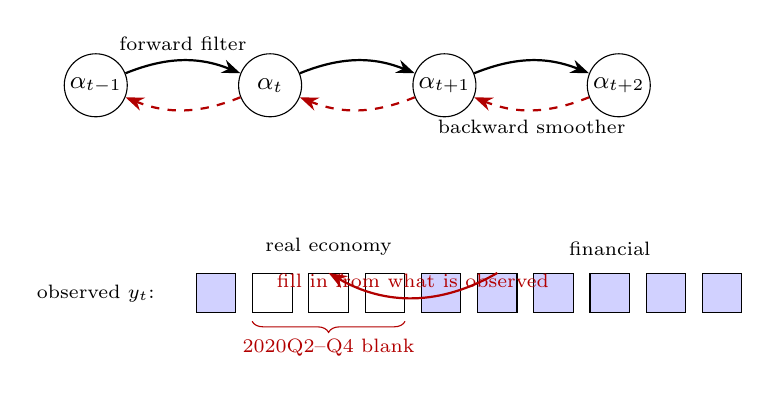
\begin{tikzpicture}[
  >=Stealth, font=\small,
  state/.style={circle,draw,minimum size=8mm,inner sep=0pt},
  obsfill/.style={rectangle,draw,minimum size=5mm,inner sep=0pt,fill=blue!18},
  obshollow/.style={rectangle,draw,minimum size=5mm,inner sep=0pt,fill=white},
  filt/.style={->,draw=black,thick},
  smth/.style={->,draw=red!70!black,thick,dashed},
  node distance=14mm,
]
  \node[state] (a1) {$\alpha_{t-1}$};
  \node[state,right=of a1] (a2) {$\alpha_{t}$};
  \node[state,right=of a2] (a3) {$\alpha_{t+1}$};
  \node[state,right=of a3] (a4) {$\alpha_{t+2}$};
  \draw[filt] (a1) to[bend left=22] node[above,font=\scriptsize]{forward filter} (a2);
  \draw[filt] (a2) to[bend left=22] (a3);
  \draw[filt] (a3) to[bend left=22] (a4);
  \draw[smth] (a4) to[bend left=22] node[below,font=\scriptsize]{backward smoother} (a3);
  \draw[smth] (a3) to[bend left=22] (a2);
  \draw[smth] (a2) to[bend left=22] (a1);
  \node[below=20mm of a1,anchor=north] (lab) {\scriptsize observed $y_t$:};
  \node[obsfill,right=4mm of lab] (m1) {};
  \node[obshollow,right=2mm of m1] (m2) {};
  \node[obshollow,right=2mm of m2] (m3) {};
  \node[obshollow,right=2mm of m3] (m4) {};
  \node[obsfill,right=2mm of m4]  (m5) {};
  \node[obsfill,right=2mm of m5] (f1) {};
  \node[obsfill,right=2mm of f1] (f2) {};
  \node[obsfill,right=2mm of f2] (f3) {};
  \node[obsfill,right=2mm of f3] (f4) {};
  \node[obsfill,right=2mm of f4] (f5) {};
  \node[above=1mm of m3,font=\scriptsize] {real economy};
  \node[above=1mm of f3,font=\scriptsize] {financial};
  \draw[decorate,decoration={brace,amplitude=4pt,mirror},red!70!black]
     ($(m2.south west)+(0,-1mm)$) -- ($(m4.south east)+(0,-1mm)$)
     node[midway,below=3pt,font=\scriptsize,red!70!black]{2020Q2--Q4 blank};
  \draw[->,red!70!black,thick] (f1.north) to[bend left=30]
     node[above,font=\scriptsize]{fill in from what is observed} (m3.north);
\end{tikzpicture}
\caption{Filling in the missing data. The model is cast in state-space form; a Kalman filter runs forward
(solid) and a smoother runs backward (dashed), so each estimate uses information from both directions. In
the observation row, over the three pandemic quarters the real-economy cells (output, prices, and the
real-economy foreign averages) are left blank while the financial cells (rates, spreads, equity) are kept,
so the blanks are reconstructed from the financial signal that markets kept providing. The same procedure
fills the future when a scenario is imposed (Section~\ref{sub:cond}): a pinned value is an observed cell,
a free value a blank.}
\label{fig:smoother}
\end{figure}

We fix the pandemic window in advance rather than letting the model find it. If we asked the estimator to
locate each economy's ``crisis'' quarters on its own, it would often latch onto the wrong episode---a 2008
trough for one economy, a 2015 commodity bust for another---so we pin the window to the three quarters
that are unambiguously the pandemic for every economy. The cost is a little rigidity for economies whose
pandemic timing differed slightly; the benefit is that the treatment is transparent, the same everywhere,
and does not quietly absorb ordinary business-cycle movements into the fill-in.

\subsection{The endogenous dominant unit}
\label{sub:endous}

The standard global VAR treats the United States as an outside anchor: it is estimated on its own, it
feeds into every other economy, but nothing feeds back into it
\citep{PesaranSchuermannWeiner2004,DeesDiMauroPesaranSmith2007}. So a shock that starts abroad, or a US
shock that bounces back through trading partners, never reaches the US model. For a scenario tool this is
a real limitation, because the feedback onto the United States is often exactly the question being asked.

We remove the limitation by giving the United States the same structure as everyone else: its own three
foreign averages and its own row in the trade-weight matrix, so it both feeds and is fed by the rest of
the world. This raises the US model from $37$ variables to $40$. The estimator starts it from a quick
no-feedback fit and then re-estimates it with its foreign averages, exactly like the other economies, so
the global channel closes back onto the economy that dominates it.

The payoff is precisely the channel a scenario tool needs. A US tightening now spreads abroad, is
partly reflected back through trading partners' demand and financial conditions, and adjusts the US path
in turn; and a shock that starts abroad can move the United States. Section~\ref{sec:scenario} measures
this channel directly, by running the same US-rate scenario with and without the feedback and taking the
difference---which is, by construction, exactly what the anchor version leaves out.

\subsection{The fiscal stock--flow block}
\label{sub:fiscal}

Six economies carry a public-finance block, and here we split the work the way fiscal analysts do
\citep{Escolano2010,IMF2013DSA}: the model forecasts the pieces of the budget, and the debt ratio then
follows by arithmetic rather than from a separate regression. This keeps the debt path consistent with the
rest of the forecast, instead of adding a debt equation that might disagree with it.

The block forecasts four things---government revenue and primary spending (both as shares of GDP), the
average interest rate the government pays on its debt, and a residual adjustment---and then rolls the debt
ratio forward by the standard identity,
\begin{equation}
  d_t = d_{t-1}\,\frac{1 + i^{\text{eff}}_t/400}{1 + g^{\text{nom}}_t/100}
        \;-\; \frac{pb_t}{4} \;+\; \frac{\text{sfa}_t}{4},
  \label{eq:debt}
\end{equation}
where $d_t$ is debt as a share of GDP, $pb_t$ the primary balance (revenue minus primary spending),
$i^{\text{eff}}_t$ the average interest rate, $g^{\text{nom}}_t$ nominal GDP growth, and the last term the
residual adjustment \citep{Bohn1998}. In words: debt grows with the interest rate, shrinks with nominal
growth, and is reduced by running a primary surplus. Interest is charged on last quarter's debt and the
ratio is scaled by this quarter's growth, following the standard official definitions. Figure~\ref{fig:fiscal}
traces the flow: the four forecast drivers on the left feed the pieces of the budget in the middle, which
roll the debt ratio forward on the right, quarter after quarter.

\begin{figure}[t]
\centering
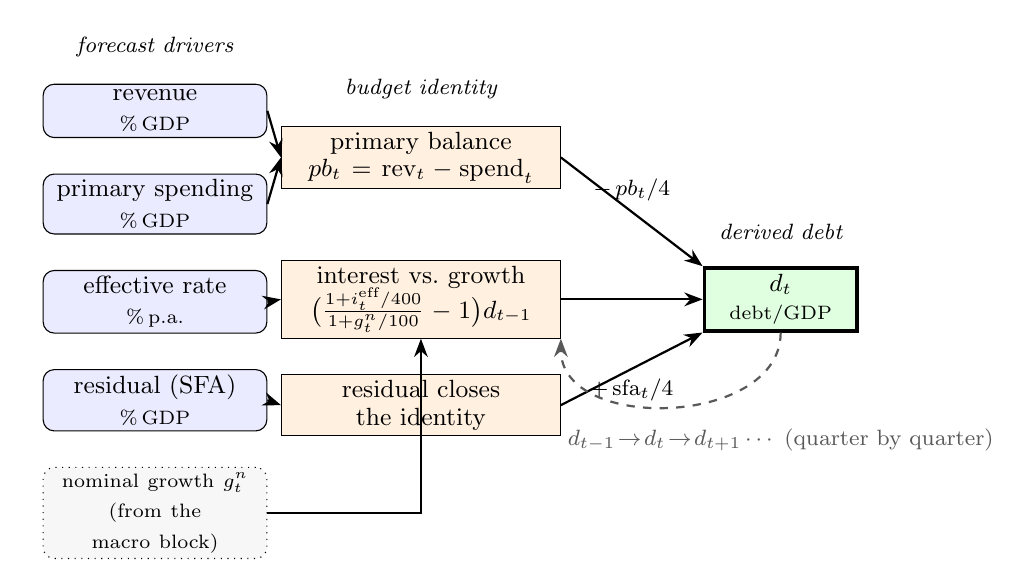
\begin{tikzpicture}[
  >=Stealth, node distance=4.5mm, font=\small,
  driver/.style={draw, rounded corners, fill=blue!8, minimum height=6.5mm, text width=27mm, align=center, inner sep=2pt},
  iden/.style={draw, fill=orange!12, minimum height=6.5mm, text width=34mm, align=center, inner sep=2pt},
  stock/.style={draw, very thick, fill=green!12, minimum height=8mm, text width=18mm, align=center, inner sep=2pt},
  op/.style={font=\footnotesize}, flow/.style={->, thick}, lag/.style={->, dashed, thick, gray!70!black},
]
  \node[driver] (rev)  {revenue\\\scriptsize \%\,GDP};
  \node[driver, below=of rev]  (exp) {primary spending\\\scriptsize \%\,GDP};
  \node[driver, below=of exp]  (eff) {effective rate\\\scriptsize \%\,p.a.};
  \node[driver, below=of eff]  (sfa) {residual (SFA)\\\scriptsize \%\,GDP};
  \node[above=2.2mm of rev, font=\footnotesize\itshape, text width=30mm, align=center] {forecast drivers};
  \coordinate (revexp) at ($(rev)!0.5!(exp)$);
  \node[iden, right=16mm of revexp] (pb) {primary balance\\[-1pt]$pb_t=\text{rev}_t-\text{spend}_t$};
  \node[iden, below=9mm of pb] (snow) {interest vs.\ growth\\[-1pt]$\bigl(\tfrac{1+i^{\text{eff}}_t/400}{1+g^{n}_t/100}-1\bigr)d_{t-1}$};
  \node[iden, below=of snow] (res) {residual closes\\[-1pt]the identity};
  \node[above=2.2mm of pb, font=\footnotesize\itshape, text width=34mm, align=center] {budget identity};
  \node[draw, dotted, rounded corners, fill=gray!6, text width=27mm, align=center, inner sep=2pt, below=of sfa]
       (gn) {\scriptsize nominal growth $g^{n}_t$\\(from the macro block)};
  \node[stock, right=18mm of snow] (dt) {$d_t$\\[-1pt]\scriptsize debt/GDP};
  \node[above=2.2mm of dt, font=\footnotesize\itshape, text width=22mm, align=center] {derived debt};
  \draw[flow] (rev.east) -- (pb.west);
  \draw[flow] (exp.east) -- (pb.west);
  \draw[flow] (eff.east) -- (snow.west);
  \draw[flow] (sfa.east) -- (res.west);
  \draw[flow] (gn.east) -| (snow.south);
  \draw[flow] (pb.east)   -- node[op, above]{$-\,pb_t/4$} (dt.north west);
  \draw[flow] (snow.east) -- (dt.west);
  \draw[flow] (res.east)  -- node[op, below]{$+\,\text{sfa}_t/4$} (dt.south west);
  \draw[lag] (dt.south) .. controls +(0,-12mm) and +(0,-12mm) .. (snow.south east);
  \node[font=\footnotesize, gray!70!black, align=center, below=11mm of dt.south, anchor=north]
       {$d_{t-1}\!\rightarrow\! d_t\!\rightarrow\! d_{t+1}\cdots$ (quarter by quarter)};
\end{tikzpicture}
\caption{The public-finance block. The model forecasts the four drivers on the left; these feed the pieces
of the government budget in the middle---revenue minus spending is the primary balance, the effective rate
against nominal growth is the interest-versus-growth term, and the residual closes the identity---which
roll the debt ratio $d_t$ forward on the right by the formula \eqref{eq:debt}, with last quarter's debt fed
back each period (dashed). Debt is computed by arithmetic, never estimated.}
\label{fig:fiscal}
\end{figure}

Because the debt path is an explicit formula in these four pieces, we can also run it backwards. Given a
target for debt, we solve \eqref{eq:debt} for the primary balance that would hit it and impose that as a
constraint (\S\ref{sub:cond}). So the same block answers both the forward question---``given this fiscal
stance, where does debt go?''---and the backward one---``what fiscal adjustment stabilises debt here?''

\subsection{The estimable fixed point and convergence}
\label{sub:fixedpoint}

The three pieces above---the country VARs, the trade links, and the data completion---are not estimated
separately; they are solved together, by repeating a simple loop until it settles. There is a
chicken-and-egg problem: to complete a country's missing data we need its partners' data, but those
partners have missing data of their own. We break it by iterating. Start with a rough guess of the
foreign averages; fill in each country's missing data given everything currently observed; rebuild the
foreign averages from the filled-in data; re-estimate each country's VAR; and repeat until the foreign
averages stop changing. This is exactly the expectation--maximization (EM) idea: the ``missing'' pieces
are the foreign series that tie the countries together, the completion step is the E-step, and the
re-estimation step is the M-step. Algorithm~1 states it precisely.

\begin{quote}
\noindent\textbf{Algorithm 1: EM--Bayesian GVAR fixed-point estimation}
(\code{pipeline/export\_bvar\_gvar24\_loop.m})
\begin{enumerate}
  \item \textbf{Bootstrap.} Form an initial guess of each foreign star from raw partner data; mask the
        COVID window $2020$Q2--Q4, setting \emph{macro only} to missing (domestic macro $+$ ROWDEM $+$
        ROWINF) and keeping all financial columns and ROWFIN observed.
  \item \textbf{E-step (DK completion).} For each bloc, run the Durbin--Koopman smoother inside the
        per-bloc sampler to impute the macro holes conditional on the observed financials, giving a
        completed panel $\widehat X_i = \E[X_i \mid \text{observed}]$.
  \item \textbf{Rebuild stars.} Recompute $y^{*}_{i,t}$ from the completed partner panels via
        \eqref{eq:stars}, renormalising weights over present partners.
  \item \textbf{M-step (Bayesian estimation).} Re-estimate each bloc \eqref{eq:bloc} by GLP Gibbs on
        $[\,\text{domestic}\mid\text{3 stars}\,]$, updating $(\widehat A_i,\widehat\Sigma_i)$ and the
        hyperparameters.
  \item \textbf{Convergence.} Stop when $\max_i\lVert \Delta y^{*}_i\rVert_\infty < \text{TOL}=0.03$
        (evaluated from the second sweep and excluding the COVID-imputed cells, whose Monte-Carlo churn
        floors around $0.13$); else return to Step~2, capped at $\text{MAXIT}=12$.
\end{enumerate}
\end{quote}

Figure~\ref{fig:emloop} draws the loop. A quick no-feedback fit of the United States seeds the first set of
foreign averages; from there each pass rebuilds the foreign averages from partners' filled-in data
(top), fills in the missing cells and re-estimates every country model (the E- and M-steps on the right and
bottom), and checks whether the foreign averages have stopped moving (left). When they have, the system
has found its joint solution and is exported.

\begin{figure}[t]
\centering
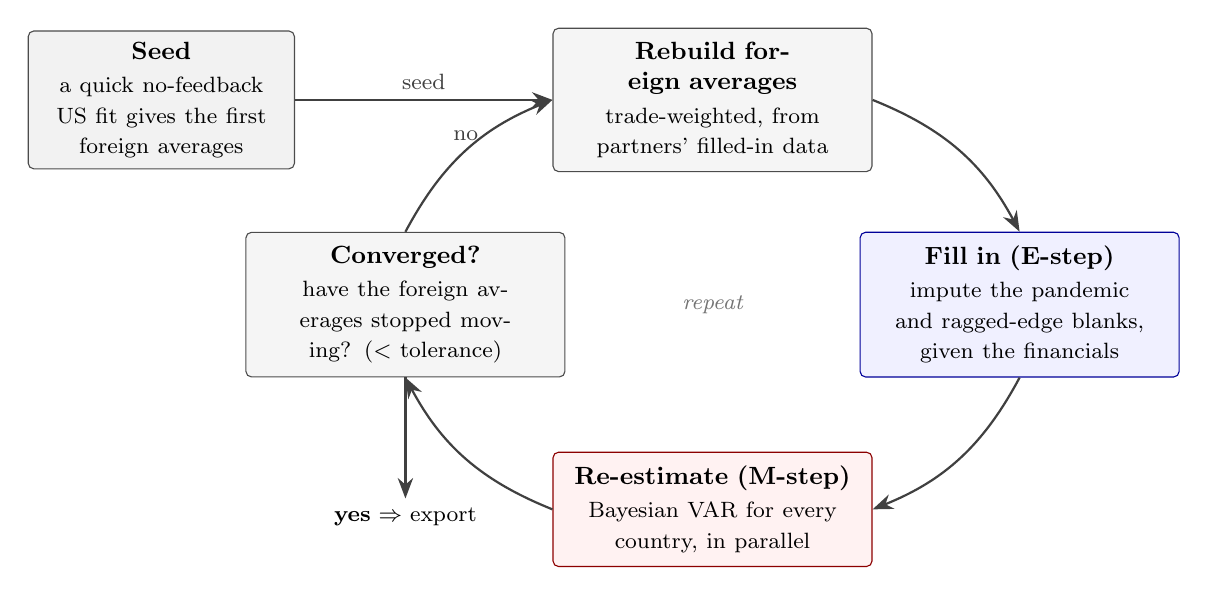
\begin{tikzpicture}[
  >={Stealth[length=2.6mm]}, font=\small,
  boot/.style={rounded corners=2pt, draw=black!70, fill=black!5, align=center, inner sep=4pt, text width=3.1cm},
  estep/.style={rounded corners=2pt, draw=blue!60!black, fill=blue!6, align=center, inner sep=5pt, text width=3.7cm},
  mstep/.style={rounded corners=2pt, draw=red!55!black, fill=red!5, align=center, inner sep=5pt, text width=3.7cm},
  box/.style={rounded corners=2pt, draw=black!70, fill=black!4, align=center, inner sep=5pt, text width=3.7cm},
  flow/.style={->, thick, black!75},
]
  \node[boot] (boot) at (-7.0,2.6) {\textbf{Seed}\\[1pt]\footnotesize a quick no-feedback US fit gives the first foreign averages};
  \node[box] (stars) at (0,2.6) {\textbf{Rebuild foreign averages}\\[1pt]\footnotesize trade-weighted, from partners' filled-in data};
  \node[estep] (estep) at (3.9,0) {\textbf{Fill in (E-step)}\\[1pt]\footnotesize impute the pandemic and ragged-edge blanks, given the financials};
  \node[mstep] (mstep) at (0,-2.6) {\textbf{Re-estimate (M-step)}\\[1pt]\footnotesize Bayesian VAR for every country, in parallel};
  \node[box] (conv) at (-3.9,0) {\textbf{Converged?}\\[1pt]\footnotesize have the foreign averages stopped moving? ($< $ tolerance)};
  \draw[flow] (boot.east) -- node[above,font=\footnotesize]{seed} (stars.west);
  \draw[flow] (stars.east)  to[bend left=20] (estep.north);
  \draw[flow] (estep.south) to[bend left=20] (mstep.east);
  \draw[flow] (mstep.west)  to[bend left=20] (conv.south);
  \draw[flow] (conv.north)  to[bend left=20] node[above,font=\footnotesize]{no} (stars.west);
  \node[align=center, font=\footnotesize] (out) at (-3.9,-2.7) {\textbf{yes} $\Rightarrow$ export};
  \draw[flow] (conv.south) -- (out.north);
  \node[font=\footnotesize\itshape, text=black!55, align=center] at (0,0) {repeat};
\end{tikzpicture}
\caption{The estimation loop. A no-feedback fit of the United States seeds the first foreign averages. Each
pass then rebuilds those averages from partners' filled-in data, fills in the missing cells and
re-estimates every country's model (the fill-in and re-estimation are the two steps of one sampler), and
checks whether the foreign averages have stopped changing. When they have, the joint solution is reached
and exported; the countries are re-estimated in parallel, which keeps a $50$-economy fit tractable.}
\label{fig:emloop}
\end{figure}

The sweep is run as a Jacobi update, which is order-independent and reaches the same fixed point as a
sequential Gauss--Seidel pass. All stars are built from the completions frozen at the start of a sweep,
then every bloc is re-estimated in parallel; this parallelism is what keeps a $50$-economy,
$1000$-draw estimation tractable. The convergence metric deliberately excludes the COVID-imputed
star cells, whose quarter-to-quarter movement is imputation Monte-Carlo noise rather than genuine
non-convergence, so the tolerance measures the systematic drift of the stars, not the sampler's variance.

The resulting system is stationary and, as Section~\ref{sec:engine} exploits, contractive. At the
deployed configuration the coupled operator has spectral radius $\rho(M)=0.947<1$, comfortably below the
stability boundary, so the cross-country fixed point is unique and the forecasts do not explode at the
$H=20$ horizon. Setting the iteration cap to one recovers a single-country mode (no star
re-convergence), which we use in Section~\ref{sec:horserace} as an ablation that isolates exactly the
value of the EM fixed point.

%% =====================================================================
\section{Real-time solution and the scenario engine}
\label{sec:engine}
%% =====================================================================

This section is the heart of the paper: it shows how the estimated model of
Section~\ref{sec:estimation} becomes an interactive tool. The idea is simple. A scenario is a linear
problem, so it can be solved once and reused (\S\ref{sub:affine}); a scenario is then just a forecast that
respects the pinned values, which a Kalman smoother produces (\S\ref{sub:cond}); users can also pin a
variable's long-run value, and the forecast glides to it (\S\ref{sub:anchor}); and because each solve is a
single matrix multiplication, the whole thing runs in a browser in milliseconds (\S\ref{sub:tool}).

\subsection{The affine fixed point and the pre-shipped inverse}
\label{sub:affine}

Once the model is estimated, imposing a scenario is a linear problem, and this is what makes the tool
fast. Hold the estimated coefficients fixed. Then each country's conditional forecast is a linear function
of the values the user pins down: doubling the size of a pinned change doubles every response, and the
\emph{pattern} of responses is unchanged. Stacking all countries together, the scenario response $x$
solves
\begin{equation}
  x = M x + d
  \qquad\Longrightarrow\qquad
  x = (I - M)^{-1} d ,
  \label{eq:coupling}
\end{equation}
where $d$ collects the user's own pinned changes and $M$ is the map that carries one country's movements
into its partners through the trade links (\code{app/src/lib/compute/gvarSolve.ts}). The countries are
tied together in \emph{deviations} from the baseline, so $M$ never has to be rebuilt from one scenario to
the next.

The key point is that $M$ depends only on the estimated model and on which variables are pinned---not on
the numbers themselves. So the answer to \emph{any} scenario that pins the same set of variables is
$x = (I-M)^{-1}d$, and we need the inverse $(I-M)^{-1}$ only once. We compute it offline, store it, and
ship it with the tool. This matters because the system is large: stacked across the $33$ coupled economies
(three lags, twenty quarters, plus the shared US-driven series) the problem has about $2{,}060$
dimensions, and inverting a matrix that size inside a browser would take close to an hour. Doing it once,
offline, turns each scenario into a single matrix multiplication that runs in milliseconds. A stored
fingerprint of the model guards the file: if the estimated model ever changes, the fingerprint no longer
matches and the tool falls back to a slower but always-correct step-by-step solve. The pre-computed
inverse is therefore not a speed trick added on top of the tool---it is what makes an interactive global
tool possible at all.

The scenario always has a unique, finite answer because the system is stable. The map $M$ keeps all of its
dynamics safely inside the unit circle: its largest eigenvalue is $0.947$, comfortably below one, so the
feedback across countries dies out rather than building up, and $(I-M)^{-1}$ is well defined.

\subsection{Conditional forecasting via the smoother}
\label{sub:cond}

A scenario is just a set of values the user fixes for the future, and the job is to fill in everything
else consistently. We do this with a standard trick: treat the future the same way we treat missing past
data \citep{DurbinKoopman2012,BanburaGiannoneLenza2015}. A value the user pins is like an observation we
happen to have for a future quarter; a value left free is like a missing observation. Running the Kalman
filter and smoother then produces the best estimate of the \emph{whole} future path consistent with the
pinned values, so fixing one variable moves all the others together rather than one at a time. As a check,
a scenario that fixes nothing reproduces the plain forecast exactly.

The user can pin a value hard or soft, which is a way of saying how sure they are. A hard pin is imposed
exactly; a soft pin is imposed only partially, so the model is allowed to disagree with it. Soft pins are
how outside forecasts---a published inflation projection, a market-implied rate path---enter as
\emph{ingredients} rather than as facts: a ``trust'' dial runs from full trust (a hard pin) to no trust
(no effect) \citep{RobertsonTallmanWhiteman2005}. The user can also pin a \emph{combination} of variables,
which is what the fiscal block uses to hit a debt target by constraining revenue minus spending.

A scenario crosses borders through the same linear system of \S\ref{sub:affine}. Pinning a variable moves
that country's trade-weighted averages away from baseline; those movements enter its partners through
$M$; each partner's smoother passes them into its own variables; and the linear solve settles all of this
at once. Because the whole thing is linear, changing the size of a pinned value re-solves all $50$
economies instantly, with no filter to re-run---which is what lets a user drag a scenario and watch every
country move in real time. For genuine policy counterfactuals the tool also offers a stricter mode that
treats the pinned rate as a policy \emph{shock} at the constrained quarters, in the spirit of
\citet{WaggonerZha1999} and \citet{AntolinDiazPetrellaRubioRamirez2021}, and lets the remaining quarters
follow the model's own dynamics.

\subsection{Long-run anchoring: a reactive steady-state prior}
\label{sub:anchor}

The user can also fix where a variable settles in the long run---say, inflation returning to two
percent---and the forecast will glide there, without re-estimating anything. This is useful because the
estimated dynamics are very persistent, so the far end of a forecast can drift to a level the user does
not believe. The textbook remedy is a prior on the long-run mean \citep{Villani2009}, but that means
re-estimating the model; a tool needs the same effect instantly, on top of the shipped model.

The idea is to nudge the forecast's long-run drift by just enough to land on the chosen value. Writing the
forecast as $Y_{T+h} = T^{h}Y_T + S_h\,c$, where $S_h=\sum_{k=0}^{h-1}T^{k}$ accumulates the model's
dynamics out to horizon $h$, a change $\delta c$ in the constant $c$ shifts the path by exactly
$S_h\,\delta c$; we pick $\delta c$ so the long-run forecast hits the target. We deliberately do not use
the model's exact long-run mean $(I-\sum_\ell A_\ell)^{-1}c$, because with such persistent dynamics that
number is unstable and unreliable; the finite-horizon quantity $S_H$ is well behaved and does the job.

One detail makes the result look right. If we applied the whole correction from the first forecast
quarter, the near term would jump---a growth variable could be pushed into a spurious recession on impact.
Instead we phase the correction in gradually, at the speed the variable's own estimated dynamics converge:
the fraction applied by horizon $h$ is
\begin{equation}
  w_j(h) = \frac{S_h[j,j]}{S_H[j,j]}, \qquad w_j(1)\approx 0, \quad w_j(H)=1,
  \label{eq:transition}
\end{equation}
zero at first and one at the end. So the forecast starts where the data leave it and drifts smoothly to
the chosen long-run value. The correction is added in the same way to the central forecast and to every
uncertainty band, so the bands keep their width---the anchor moves the central view without pretending to
add certainty.

\subsection{From estimation apparatus to interactive tool}
\label{sub:tool}

Because each new scenario is a single matrix multiplication, the whole $50$-economy model runs inside the
browser and answers in a fraction of a second. The files it needs---the estimated country models, the
pre-computed inverse, and the response tables---are shipped with the web page; imposing or dragging a
scenario triggers the multiplication and a quick pass of the smoother, with no re-estimation and no trip
to a server. An analyst can therefore explore a scenario interactively, tightening or loosening a
constraint and watching all $50$ economies move.

Shipping the model this way also makes it reproducible. Every number the user sees comes from a shipped
file and a documented calculation, and the files carry a fingerprint of the estimated model, so anyone can
check that the tool is running the model this paper describes. The forecasting test of
Section~\ref{sec:horserace} and the scenarios of Section~\ref{sec:scenario} use these same files, so the
paper's evidence and the live tool are one and the same.

%% =====================================================================
\section{Data}
\label{sec:data}
%% =====================================================================

The system runs on a harmonised quarterly panel of $50$ economies and $1{,}182$ series drawn from
official statistical sources. The $33$ GVAR-coupled blocs span the United States, the euro area as an
aggregate, the other major advanced economies, and a broad set of emerging markets; a further $17$
euro-area members are estimated as standalone models that carry the common euro-area instruments as
external regressors. Appendix~\ref{app:roster} lists the full roster with each bloc's variable count and
sample.

The variable set per bloc spans a macro core, a financial/credit block, and---for $42$ economies---a
fiscal block. The macro core is real GDP and its expenditure components, price deflators and consumer
prices, unemployment, a short rate, a long yield, and a nominal effective exchange rate; the financial
block adds a corporate spread, equity, a house-price index, and non-financial-corporate credit; the
fiscal block adds the four drivers of Section~\ref{sub:fiscal}. Sources are the standard official
providers---Eurostat, the OECD, the BIS, the Federal Reserve's FRED, the ECB, the IMF, and national
government-finance statistics---documented per series in the shipped coverage manifest.

Estimation samples are genuinely ragged, and the system uses each series' true span rather than a
truncated common window. Advanced economies reach back furthest (the United States to $1998$, the
euro-area members to around $2000$), while several emerging markets begin only in the late $2000$s or
$2010$s; the EM data-completion of \S\ref{sub:em} is precisely what lets these unequal spans coexist in
one coupled system. All blocs share a common last estimation quarter, and the coupling aligns them by
projection step rather than by calendar date, so a bloc whose data ends a quarter early is completed by
one coupled conditional solve rather than by dropping a quarter from every other bloc.

We are explicit about data provenance and its limits, and scope the empirical claims accordingly. A small
number of blocs carry a model-extended tail (the last few quarters filled by a temporal-disaggregation
step) or a proxy for a variable that is not directly available at quarterly frequency; these are
documented per bloc in the project's data audit. Accordingly, Section~\ref{sec:horserace} draws its
headline conclusions from the clean anchor blocs (US, EA, JP, UK, CA) whose panels are genuinely observed
throughout, and reports the full $33$-bloc panel in Appendix~\ref{app:fullpanel} with the model-extended
blocs flagged. The pandemic window is carried as missing data rather than removed or dummied, consistent
with \S\ref{sub:em}, and is therefore not a provenance caveat but a modelling choice.

%% =====================================================================
\section{Does it forecast? The out-of-sample credibility floor}
\label{sec:horserace}
%% =====================================================================

Before we ask the model to support scenarios, we check that it forecasts credibly, so that the scenarios
in Section~\ref{sec:scenario} rest on more than a nice picture. We set the bar as a floor, not a
leaderboard: the question is not whether the model wins, but whether it holds its own against the best
available models and clearly beats the textbook global VAR it generalizes.

\subsection{Design}
\label{sub:eval-design}

We test the model the way it would actually have been used: at a sequence of past dates, using only the
data available at the time, and comparing its forecasts against those that later came true. We run the
experiment from $2010$Q1 to $2024$Q4, re-estimating every model on the data up to each date and
forecasting to $h\in\{1,2,4,8\}$ quarters ahead; the four $2020$ dates are dropped as an outlier the
exercise is not about. One honest limitation sets in at the early dates: the model carries a credit block,
and credit history is short, so before about $2013$ the credit-augmented model cannot be estimated
reliably and simply does not enter---the effective evaluation window is roughly the eleven years
$2013$--$2024$. This is a genuine feature of the model, not a bug, and it is why we compare all models only
on the dates they all share. We report the clean anchor blocs (US, EA, JP, UK, CA) for growth, inflation,
and the short interest rate, and put the full $33$-economy panel in Appendix~\ref{app:fullpanel}. The
pandemic-as-missing treatment still applies within each estimation, so the model faces the same ragged,
pandemic-scarred data in the test as it does in use.

The single most important design choice is that the trade weights are recomputed at each date from data
up to that date only. This is the main guard against letting the model peek at the future: a forecast made
in $2012$ never uses the trade patterns of $2021$. The trade weights shipped with the tool, which average
a recent period, are not allowed in the test. Three further guards go with it---each model sees only data
up to the forecast date, the cross-country loop re-converges on that data alone, and nothing is adjusted
after the fact---so the test genuinely mimics how the model would have been run in real time.

The set of competitors runs from the very simple to the textbook global VAR, and includes two
stripped-down versions of our own model that show what each ingredient adds (Table~\ref{tab:bench}). A
random walk is the universal reference; an autoregression is a strong single-variable benchmark; a
single-country Bayesian VAR removes the trade links, so the comparison with it shows what \emph{linking
the countries} buys; the textbook global VAR is the literature's standard, so beating it shows what the
Bayesian estimation and data-completion buy; a single-pass version of our model (one iteration of the
loop) shows what \emph{iterating to convergence} buys; and a dynamic factor model asks whether the global
VAR structure is needed at all. Against these stand the two versions of our model---with the United States
responding to the world (the deployed one) and with it held as a fixed anchor.

\begin{table}[t]
\centering
\caption{The nine-model out-of-sample suite: two proposed variants, six benchmarks, and a climatology
sibling of the random walk. The two ablations (\code{cgvar\_b}, \code{sbvar}) isolate the EM fixed point
and the coupling respectively.}
\label{tab:bench}
\begin{tabular}{@{}lll@{}}
\toprule
Model (id) & Cross-country structure & Role / ablation \\
\midrule
Random walk (\code{rw}, +\,\code{rw\_clim})   & none                       & universal reference \\
AR($p$) (\code{arp})                          & none                       & strong univariate dynamic \\
Single-country BVAR (\code{sbvar})            & none (per-bloc GLP)        & value of \emph{coupling} \\
Textbook OLS GVAR (\code{cgvar\_a})           & fixed weights, exog.\ US, OLS & value of the Bayesian$+$EM apparatus \\
Single-pass Bayesian GVAR (\code{cgvar\_b})   & coupled, $\text{MAXIT}=1$  & value of the \emph{EM star fixed point} \\
Dynamic factor model (\code{dfm})             & static factors             & ``is the GVAR structure needed?'' \\
\textbf{EM--Bayesian GVAR, frozen (\code{emgvar\_frozen})} & coupled, exog.\ US & legacy anchor \\
\textbf{EM--Bayesian GVAR, endog.\ (\code{emgvar\_endo})}  & coupled, endog.\ US & the deployed system \\
\bottomrule
\end{tabular}
\end{table}

\subsection{Scoring and inference}
\label{sub:eval-scoring}

We judge the models in two ways. For point accuracy we use the root-mean-squared forecast error, reported
relative to the random walk, so a number below one means ``better than the naive benchmark.'' For the full
probability forecast we use the continuous ranked probability score, or CRPS, a standard measure of how
well a predicted distribution matches what actually happened \citep{GneitingRaftery2007}. Our main way of
ranking models is the Model Confidence Set \citep{HansenLundeNason2011}: for each variable and horizon it
returns the group of models that are statistically tied for best, so a model earns credit not for winning
outright but for belonging to that group.

For the individual comparisons we use the tests that are valid for this setup---forecasts from models that
often nest one another, re-estimated on a growing sample. Giacomini--White \citep{GiacominiWhite2006}
carries the main comparisons; Clark--West \citep{ClarkWest2007} is used when one model is a special case of
another; Diebold--Mariano \citep{DieboldMariano1995,HarveyLeybourneNewbold1997} for models that do not nest;
and a Romano--Wolf step-down \citep{RomanoWolf2005} keeps the overall error rate under control when we make
many comparisons at once. We also check whether the probability bands are the right width, using the
probability-integral transform.

One scoring choice is forced on us, and we are open about it. The natural score for a probability
forecast, the log-score, turns out to be numerically unusable here: our forecasts are clouds of
simulation draws, and scoring them with a fitted bell curve blows up on the fat-tailed pandemic-era draws.
Following the density-forecast literature \citep{AmisanoGiacomini2007} we therefore rely on the CRPS and
the Model Confidence Set, which do not suffer from this problem, and set the log-score aside.

\subsection{Results}
\label{sub:eval-results}

We report three results. First, the model does not win on point accuracy, and we say so plainly. On
squared error, the factor model forecasts growth best at every horizon, and the autoregression forecasts
inflation and the short interest rate best at the shorter horizons. This is what one expects of a large
linked model: its value is a consistent picture across many economies, not the smallest error on any one
series.

Second, once we judge the whole probability forecast, the model is in the tied-for-best group almost
everywhere. By the Model Confidence Set (scored on the density, the CRPS), our model is statistically
indistinguishable from the best available for growth at every horizon, for inflation at every horizon, and
for the short rate up to one year ahead; it drops out only for the short rate at the longest horizons
(Table~\ref{tab:mcs}). We are careful not to over-read this. On the window the credit-augmented model can
be estimated (about eleven years, discussed in \S\ref{sub:eval-design}), the confidence sets are wide, so
several models---including the textbook global VAR---survive in many cells. The Model Confidence Set tells
us our model is not distinguishable from the best; the sharper question is whether it beats the specific
model it generalizes, which we take up next.

Third, against the textbook OLS global VAR---the model ours generalizes---the extra machinery pays off on
the real side. A direct accuracy test on the density (Giacomini--White on the CRPS) shows our model
significantly beats the textbook version on growth (decisively one quarter ahead, and again at one and two
years) and on inflation at the longer horizons; the one place the textbook version holds its own is the
short interest rate at longer horizons. So the Bayesian estimation, the pandemic-as-missing completion,
and the cross-country loop earn their place chiefly on growth and inflation---a more measured claim than an
across-the-board win, and the honest one.

\begin{table}[t]
\centering
\caption{$90\%$ Model Confidence Set membership (density/CRPS), anchor blocs, over the estimable window.
\checkmark{} $=$ statistically indistinguishable from the best. The sets are wide on this window (several
models survive per cell), so this establishes that the model is \emph{among} the best rather than the
uniquely best; the pairwise test against the textbook global VAR (text) is the sharper comparison.}
\label{tab:mcs}
\begin{tabular}{@{}lcccc@{}}
\toprule
& \multicolumn{4}{c}{horizon $h$} \\
\cmidrule(l){2-5}
Target ($\to$ our model) & 1 & 2 & 4 & 8 \\
\midrule
Growth     & \checkmark & \checkmark & \checkmark & \checkmark \\
Inflation  & \checkmark & \checkmark & \checkmark & \checkmark \\
Short rate & \checkmark & \checkmark & ---        & --- \\
\bottomrule
\end{tabular}
\end{table}

A separate comparison concerns our own two versions. With the United States responding to the world, and
with it held as a fixed anchor, the two are statistically indistinguishable as \emph{forecasters}:
endogenizing the United States does not sharpen the forecast. Its value is the scenario feedback of
Section~\ref{sec:scenario}, which the fixed anchor cannot produce at all---so the two variants are a wash
here and part company only when the model is used as a scenario tool.

One weakness is clear and we report it openly: the model's probability bands are too narrow. Its
$90\%$ bands actually cover the outcome about $74$--$82\%$ of the time, short of the $90\%$ they claim, and
the gap is worst one quarter ahead. The reason is that the forecast carries the usual shock and
parameter uncertainty but leaves out the extra uncertainty from having filled in the pandemic quarters. We
therefore lean on the CRPS and the Model Confidence Set, which are not thrown off by this, and we flag the
fix---feeding the fill-in uncertainty into the bands---in Section~\ref{sec:discussion}. These are
sweep-quality results; a final pass with more posterior draws should tighten the bands further.

\subsection{What the test establishes}
\label{sub:eval-summary}

The point is not a win but a floor. Linking the countries, shrinking the estimates, and filling in the
missing data together deliver forecasts that sit inside the best group on growth, inflation, and the short
rate, and that significantly beat the textbook global VAR on growth and inflation. That is what the
scenario application needs: a model whose forecasts we can trust well enough to believe the way it
propagates a scenario. We turn to that next.

%% =====================================================================
\section{What it enables: global scenario analysis}
\label{sec:scenario}
%% =====================================================================

The point of the tool is the analysis it makes easy: fast, consistent what-if projections across all the
economies at once. Section~\ref{sec:horserace} asked whether the model forecasts; this section shows what
using it as a tool adds---scenarios that hang together across $50$ economies, are quick enough to explore
live, and carry their public-debt consequences automatically.

\subsection{A scenario is just a conditional forecast}
\label{sub:scenario-def}

Here a scenario is not a set of paths adjusted by hand. It is a forecast of the whole $50$-economy system
that respects a few values the user fixes. The user fixes what the scenario says---a policy rate held
above its baseline, a credit spread widened, a budget loosened---and the engine of \S\ref{sub:cond}
reports the implied path of every other variable in every economy, consistent with the estimated dynamics
and the trade links. Nothing is touched by hand afterward, so two analysts who set the same values get the
same global picture.

We draw our scenarios from a documented library of policy-relevant shocks. Four are the mainstays: a jump
in corporate borrowing spreads with a flight to safe bonds, a global energy-supply shock, a budget
loosening that widens deficits, and a monetary policy that falls behind the curve. Each is written as a
small set of fixed values with a sourced rationale, and each runs through the same engine, so the library
is a set of inputs to one model rather than a collection of separate models.

\subsection{A global transmission exhibit}
\label{sub:scenario-transmission}

A US interest-rate rise reaches every economy in one solve. Fixing the US policy rate above its baseline
tightens US financial conditions, which pass through the trade links and the globally-traded prices to
every partner: the euro area and the other advanced economies tighten alongside the United States,
emerging markets with strong dollar links tighten more, and the resulting pattern of growth and inflation
across economies is the consistent global picture the tool draws in real time
(Figure~\ref{fig:ea-spillover}). Re-run with the rate raised or lowered, the same solve updates every
economy at once---which is what makes the tool usable in a meeting.

\begin{figure}[t]
\centering

\includegraphics[width=0.82\textwidth]{manual_figs/ui_gvar_ea.png}
\caption{The euro-area view after a US tightening scenario is solved through the linked system: the
domestic paths (central line and uncertainty band) respond to the US rate through the trade links and the
globally-traded prices. Drawn in the browser from the pre-computed files.}
\label{fig:ea-spillover}
\end{figure}

\subsection{The feedback onto the United States}
\label{sub:scenario-endous}

Letting the United States respond to the rest of the world adds a feedback that the fixed-anchor version
cannot produce, and we measure it by running the very same US-rate scenario both ways. We hold the US
policy rate $100$ basis points above baseline for the whole horizon and solve twice from identical inputs:
once with the United States responding to the world, and once with it held as a fixed anchor (which we
obtain by removing the three US foreign-average terms, leaving everything else byte-for-byte the same, so
the difference reflects only the feedback). With the anchor, the US path is driven purely by its own
dynamics; with the feedback on, the rest of the world loops back onto the US.

The gap between the two, endogenous minus frozen, is the feedback the frozen GVAR structurally omits
(Table~\ref{tab:spillover}). With the anchor, the United States gets no feedback, so its growth and
inflation move only through its own dynamics; letting it respond adds the loop from the rest of the world,
and the difference---about $1$ to $2$ points at the peak, and of mixed sign across the six economies---is
the size of that loop. We are careful about these numbers for two reasons. First, holding the US rate
$100$ basis points high for the whole horizon is a scenario projection, not a one-off policy shock or an
impulse response \citep{PesaranShin1998}: because high interest rates tend to go together with strong
activity in the data, as much as they cause weak activity, some of the individual responses come out with
a counter-intuitive sign---which is exactly why we do not call this a shock. Second, the \emph{difference}
is cleaner than the individual responses, because it cancels the own-dynamics that both versions share, but
its sign and pattern still depend on the estimated trade links. So the qualitative message is solid---
letting the United States respond adds a real feedback the fixed anchor cannot---while pinning down the
numbers needs a proper impulse-response and connectedness calculation \citep{DieboldYilmaz2012}, which we
leave to future work. The run also serves as a check on the solver: the fast (pre-computed-inverse) solve
matches the slow step-by-step solve to within $10^{-4}$ for every economy, and the fixed-anchor version is
stable (largest eigenvalue $0.70$, against $0.947$ for the full linked system).

\begin{table}[t]
\centering
\caption{US $+100$\,bp conditional projection on the deployed system: peak (max-abs) scored-space response
by bloc and topology, and the endogenous$-$frozen gap. The gap is the Rest-of-World$\to$US feedback
channel, absent under the frozen anchor. Individual own-responses inherit the reduced-form
projection confound and are not causally interpretable; the gap differences it out. Scored space is
$4\Delta$(level) for growth/inflation.}
\label{tab:spillover}
\begin{tabular}{@{}llrrr@{}}
\toprule
Bloc & Var & endo & frozen & gap \\
\midrule
US & growth & $+1.80$ & $+2.15$ & $-1.97$ \\
   & infl   & $+0.71$ & $+1.11$ & $-1.09$ \\
EA & growth & $+1.53$ & $+1.32$ & $-1.31$ \\
   & infl   & $+0.91$ & $+0.55$ & $-1.06$ \\
JP & growth & $+1.91$ & $+1.50$ & $-1.52$ \\
   & infl   & $+1.22$ & $+0.69$ & $+1.14$ \\
UK & growth & $+1.57$ & $+1.89$ & $+1.63$ \\
   & infl   & $+0.77$ & $+0.74$ & $-0.97$ \\
CA & growth & $+1.02$ & $+1.10$ & $+0.81$ \\
   & infl   & $+2.05$ & $-0.97$ & $+1.74$ \\
CN & growth & $+3.12$ & $+2.21$ & $-1.66$ \\
   & infl   & $-0.59$ & $+1.20$ & $-1.50$ \\
\bottomrule
\end{tabular}
\end{table}

\subsection{The fiscal/debt response}
\label{sub:scenario-fiscal}

A scenario's debt consequences come for free, because the debt path is computed from the forecast. When a
scenario moves growth, inflation, and the interest rate the government pays, the debt formula
\eqref{eq:debt} turns them into a debt path with no extra modelling: a tightening that raises the interest
rate and slows growth pushes debt up, and the tool draws the resulting debt path next to the growth and
inflation charts (Figure~\ref{fig:debt}). Run backwards, the same formula answers the other question a
policymaker asks---if we want debt to stabilize here, what fiscal adjustment does that take?---so both the
``what happens'' and the ``what would it take'' come out of one scenario.

\begin{figure}[t]
\centering

\includegraphics[width=0.82\textwidth]{manual_figs/ui_debt_panel.png}
\caption{The derived debt block responding to a tightening scenario: the debt ratio follows from the
budget identity \eqref{eq:debt} given the scenario's growth, inflation, and effective-rate paths, so the
debt-sustainability implication is automatic rather than separately modelled.}
\label{fig:debt}
\end{figure}

%% =====================================================================
\section{What the system enables; limitations}
\label{sec:discussion}
%% =====================================================================

The two parts of the paper together make one point: a single model does both jobs, in real time, from one
reproducible set of files. The forecasting test shows the model sits among the best on growth, inflation,
and interest rates and significantly beats the textbook global VAR on growth and inflation; the scenario
application shows the same model produce consistent what-if projections across $50$ economies and a genuine
feedback onto the United States that a fixed anchor cannot. Neither the forecasting nor the scenario side
is new on its own; carrying both in one model that anyone can inspect and re-run is.

Having one model for both lowers the cost of coherent global policy analysis. An institution that would
otherwise run a forecasting model and a separate scenario setup---and reconcile the two by hand---can
instead fix a few values in one model and read a globally consistent answer, with the debt implications
attached. And because everything ships as files with a documented calculation behind each number, the
analysis can be audited.

We are open about the current limitations. The probability bands are too narrow, because the forecast
leaves out the uncertainty from filling in the pandemic quarters, so we read the density results through
the CRPS and the Model Confidence Set rather than at face value. The feedback onto the United States is a
scenario projection, not a causal impulse response, and pinning down its size needs the impulse-response
calculation we have not yet done. And a few economies carry model-extended tails or proxy series, which is
why the headline forecasting test uses the clean economies and flags the rest.

Each limitation has a clear fix. Feeding the fill-in uncertainty into the forecast would widen the bands
to the right size; adding an impulse-response and connectedness calculation would turn the US feedback
from a scenario projection into a causal statement; and re-estimating the few model-extended economies on
clean data would extend the forecasting results to the whole panel. None of these changes the design of
the model; each sharpens one piece.

%% =====================================================================
\section{Conclusion}
\label{sec:conclusion}
%% =====================================================================

Policy institutions need to answer multi-country what-if questions quickly and consistently, but the tools
to do it---Bayesian shrinkage, cross-country linking, conditional forecasting, and a careful treatment of
missing data---have existed only separately. This paper puts them together in one model, an EM--Bayesian
global VAR in which the United States responds to the rest of the world, and turns that model into a tool
by using one fact: once the model is estimated, a scenario is a linear problem, so its answer can be
pre-computed and reused, and any scenario re-solves all $50$ economies in a browser in a fraction of a
second.

The evidence comes in two parts, and we report it honestly. Out of sample the model does not win on point
accuracy, but on growth, inflation, and interest rates it is statistically among the best, and it
significantly beats the textbook global VAR it generalizes on growth and inflation---though its
probability bands come out too narrow. Letting the United States respond to the world does not sharpen the
forecast (the two variants tie); its payoff is elsewhere. As a scenario tool the model spreads global
shocks consistently across every economy, carries their debt consequences automatically, and captures a
feedback onto the United States that a fixed anchor cannot---which is where making the United States
endogenous earns its keep. The contribution is the whole system: one model, fast and reproducible, that
both forecasts credibly and supports coherent multi-country scenario analysis.

%% =====================================================================
\appendix
\section{Estimation and solution details}
\label{app:estimation}
The per-bloc sampler, the Metropolis--Hastings update of the shrinkage hyperparameters, the convergence
diagnostics of the EM sweep, and the offline precomputation of the coupling inverse are documented in full
in the technical and user manual attached at the end of this document, and reproduced by the shipped
pipeline (\code{pipeline/export\_bvar\_gvar24\_loop.m}, \code{app/scripts/precompute\_gvar\_coupling.mjs}).

\section{Data roster and per-bloc variable tables}
\label{app:roster}
Table~\ref{tab:roster} lists every economy in the panel: its variable count, whether it is a coupled
GVAR bloc, whether it carries a fiscal block, whether it carries the shared external instruments, and its
estimation sample. The table is generated directly from the shipped model specifications, so it is
accurate by construction; the per-bloc variable tables (identifier, description, transformation, prior,
block) are produced by the same script (\code{docs/generate\_manual\_tables.py}) and are available in the
online supplement.

\begin{longtable}{@{}llrcccl@{}}
\caption{The deployed panel: $50$ economies, $1{,}182$ estimated series. ``Coupled'' marks the $33$ GVAR
blocs; the other $17$ are euro-area members estimated as standalone models with the euro-area instruments
as external regressors. ``Fiscal'' marks the $42$ economies with a fiscal block; ``External'' marks the
three blocs (US, EA, CN) that carry shared instruments used by other blocs.}
\label{tab:roster}\\
\toprule
Code & Economy & $n$ & Coupled & Fiscal & External & Sample \\
\midrule
\endfirsthead
\multicolumn{7}{@{}l}{\emph{\ldots continued}}\\
\toprule
Code & Economy & $n$ & Coupled & Fiscal & External & Sample \\
\midrule
\endhead
\bottomrule
\endlastfoot
\texttt{AR} & Argentina & 20 & \checkmark &  &  & 2004Q1--2025Q4 \\
\texttt{AU} & Australia & 25 & \checkmark & \checkmark &  & 1999Q1--2025Q4 \\
\texttt{BR} & Brazil & 24 & \checkmark & \checkmark &  & 2012Q2--2025Q4 \\
\texttt{CA} & Canada & 27 & \checkmark & \checkmark &  & 1998Q1--2025Q4 \\
\texttt{CL} & Chile & 25 & \checkmark & \checkmark &  & 2000Q1--2025Q4 \\
\texttt{CN} & China & 22 & \checkmark & \checkmark & \checkmark & 1999Q1--2025Q4 \\
\texttt{CO} & Colombia & 26 & \checkmark & \checkmark &  & 2005Q1--2025Q4 \\
\texttt{CR} & Costa Rica & 20 & \checkmark & \checkmark &  & 2010Q3--2025Q4 \\
\texttt{CZ} & Czechia & 25 & \checkmark & \checkmark &  & 2000Q1--2025Q4 \\
\texttt{DK} & Denmark & 26 & \checkmark & \checkmark &  & 2000Q1--2025Q4 \\
\texttt{EA} & Euro area & 25 & \checkmark & \checkmark & \checkmark & 1999Q1--2025Q4 \\
\texttt{HU} & Hungary & 25 & \checkmark & \checkmark &  & 2000Q1--2025Q4 \\
\texttt{IS} & Iceland & 21 & \checkmark &  &  & 2000Q2--2025Q4 \\
\texttt{IN} & India & 21 & \checkmark &  &  & 2011Q4--2025Q4 \\
\texttt{ID} & Indonesia & 24 & \checkmark & \checkmark &  & 2005Q3--2025Q4 \\
\texttt{IL} & Israel & 25 & \checkmark & \checkmark &  & 2000Q1--2024Q4 \\
\texttt{JP} & Japan & 25 & \checkmark & \checkmark &  & 2000Q1--2025Q4 \\
\texttt{KR} & Korea & 25 & \checkmark & \checkmark &  & 2000Q1--2025Q4 \\
\texttt{MY} & Malaysia & 21 & \checkmark &  &  & 2015Q1--2025Q4 \\
\texttt{MX} & Mexico & 26 & \checkmark & \checkmark &  & 2001Q4--2025Q4 \\
\texttt{NZ} & New Zealand & 25 & \checkmark & \checkmark &  & 2000Q1--2025Q4 \\
\texttt{NO} & Norway & 24 & \checkmark & \checkmark &  & 2000Q1--2025Q4 \\
\texttt{PL} & Poland & 25 & \checkmark & \checkmark &  & 2000Q1--2025Q4 \\
\texttt{RU} & Russia & 17 & \checkmark &  &  & 2003Q1--2025Q4 \\
\texttt{SA} & Saudi Arabia & 18 & \checkmark &  &  & 2010Q1--2025Q4 \\
\texttt{ZA} & South Africa & 25 & \checkmark & \checkmark &  & 2002Q1--2025Q4 \\
\texttt{SE} & Sweden & 26 & \checkmark & \checkmark &  & 2000Q1--2025Q4 \\
\texttt{CH} & Switzerland & 20 & \checkmark &  &  & 2000Q1--2025Q4 \\
\texttt{TR} & T\"urkiye & 23 & \checkmark & \checkmark &  & 2000Q1--2025Q4 \\
\texttt{TW} & Taiwan & 20 & \checkmark &  &  & 1997Q1--2025Q4 \\
\texttt{TH} & Thailand & 26 & \checkmark & \checkmark &  & 2003Q1--2025Q4 \\
\texttt{UK} & United Kingdom & 27 & \checkmark & \checkmark &  & 1997Q1--2025Q4 \\
\texttt{US} & United States & 40 & \checkmark & \checkmark & \checkmark & 1998Q3--2025Q4 \\
\midrule
\texttt{AT} & Austria & 23 &  & \checkmark &  & 2000Q1--2025Q4 \\
\texttt{BE} & Belgium & 23 &  & \checkmark &  & 2000Q1--2025Q4 \\
\texttt{DE} & Germany & 22 &  & \checkmark &  & 2000Q1--2025Q4 \\
\texttt{EE} & Estonia & 23 &  & \checkmark &  & 2000Q1--2025Q4 \\
\texttt{ES} & Spain & 23 &  & \checkmark &  & 2000Q1--2025Q4 \\
\texttt{FI} & Finland & 23 &  & \checkmark &  & 2000Q1--2025Q4 \\
\texttt{FR} & France & 23 &  & \checkmark &  & 2000Q1--2025Q4 \\
\texttt{GR} & Greece & 22 &  & \checkmark &  & 2000Q1--2025Q4 \\
\texttt{IE} & Ireland & 23 &  & \checkmark &  & 2000Q1--2025Q4 \\
\texttt{IT} & Italy & 23 &  & \checkmark &  & 2000Q1--2025Q4 \\
\texttt{LT} & Lithuania & 23 &  & \checkmark &  & 2000Q1--2025Q4 \\
\texttt{LU} & Luxembourg & 23 &  & \checkmark &  & 2000Q1--2025Q4 \\
\texttt{LV} & Latvia & 22 &  & \checkmark &  & 2000Q1--2025Q4 \\
\texttt{NL} & Netherlands & 23 &  & \checkmark &  & 2000Q1--2025Q4 \\
\texttt{PT} & Portugal & 23 &  & \checkmark &  & 2000Q1--2025Q4 \\
\texttt{SI} & Slovenia & 23 &  & \checkmark &  & 2000Q1--2025Q4 \\
\texttt{SK} & Slovakia & 23 &  & \checkmark &  & 2000Q1--2025Q4 \\
\end{longtable}

\section{Full 33-bloc evaluation panel}
\label{app:fullpanel}
The headline evaluation of Section~\ref{sec:horserace} is scoped to the clean anchor blocs; this appendix
reports the median and inter-quartile range of relative RMSE and the MCS membership across all $33$
coupled blocs, with the model-extended blocs explicitly flagged.

\section{Replication}
\label{app:replication}
The evaluation harness is a separate repository that references the main tool without copying estimator
code; given the shipped artifacts and the trade-weight caches it reproduces the horse-race and the
Tier-A spillover, and the model signature ties the reproduced results to the deployed system.

\bibliographystyle{plainnat}
\bibliography{references}

\clearpage
\phantomsection
\addcontentsline{toc}{section}{Appendix: The Technical and User Manual}
\section*{Appendix: The Technical and User Manual}
\label{app:manual}
The remainder of this document reproduces the system's technical and user manual. It gives, in full, the
detail behind every summary in the body: the exact equations of the estimator and the real-time solver,
the state-space and conditioning machinery, the fiscal accounting, the data sources and transformations
for every economy, the numerical constants of the deployed engine, and a guided tour of the tool's
interface. The paper is self-contained without it; the manual is attached so that every modelling and
implementation choice is documented and reproducible in one place.


\includepdf[pages=-,pagecommand={},fitpaper=true]{MFFM_User_Manual.pdf}

\end{document}
